\documentclass[11pt,a4paper]{article}

\usepackage{amsmath} %for mathemathic formulas
\usepackage{amssymb}
\usepackage[ngerman]{babel} %for the german language by the spellling reform (without the package the date would look like April 20, 2020)
\usepackage{enumitem} %for enumeration surrounding
\usepackage{graphicx} %for pictures
\usepackage{siunitx}

\title{Blatt 4}
\date{\today}
\author{Hannah Rotgeri \and Lena Olbrich}

\begin{document}
    \maketitle

    \section*{Aufgabe 1}
Aufgabenteile b)-f) wurden
wegen Unklarheiten nicht bearbeitet.
 

	\begin{itemize}
		\item[a)] Wurde implementiert und erfolgreich getestet.
		\item[c)] Wurde implementiert, jedoch nicht erfolgreich getestet.
		\item[d)] Wurde implementiert, jedoch nicht erfolgreich getestet.  
	\end{itemize}
 
	\begin{figure}[h]
		\centering
		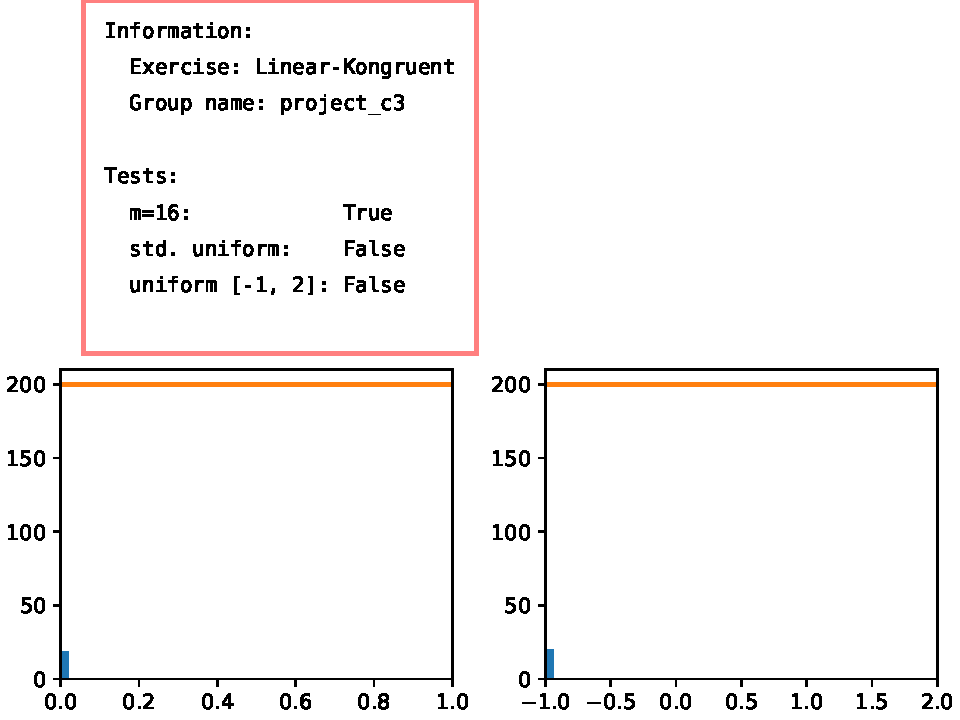
\includegraphics[width=\textwidth]{lcg.pdf}
		\caption{Ergebnis der Testdatei.}
	\end{figure}

	\section*{Aufgabe 6: Gleichverteilung}

	Zur Erzeugung der Zufallszahlen, die der entsprechenden Verteilung folgen,
	wird die Methode der Transformation der Gleichverteilung aus der Vorleusung verwendet.
	Dazu wird analog des Bespiels auf Folie 23 vorgegangen.

	\begin{itemize}
		\item[a)] Exponentialverteilung

		Normieren: $1 = N\cdot \int_0^{\infty} exp(-t/\tau)dt = [-N \tau exp(-t/\tau)]_0^{\infty} = N \tau
					\to N = 1/\tau $

		Fläche bis Zufallsvariable: $A(t) = \int_0^{t} exp(-t/\tau)dt = - \tau \cdot exp(-t/\tau) + \tau $

		Normierte Fläche: $r(t) = A(t) \cdot N = 1 - exp(-t/\tau)$

		Invertierung: $t(r) = -\tau \cdot ln(1-r)$ \to Formel zu Erzeugung der gesuchten Zufallszahlen \to im Code implementiert


		\item[b)] Potenzverteilung mit negativem Index

		Normieren: $1 = N\cdot \int_{x_{min}}^{x_{max}} x^{-n}dx = [N \cdot \frac{x^{1-n}}{1-n}]_{x_{min}}^{x_{max}} = \frac{N}{1-n} (x_{max}^{1-n} - x_{min}^{1-n})
					\to N = \frac{1-n}{x_{max}^{1-n} - x_{min}^{1-n}} $

		Fläche bis Zufallsvariable: $A(x) = \int_{x_{min}}^{x} x^{-n}dx = \frac{x^{1-n} - x_{min}^{1-n}}{1-n} $

		Normierte Fläche: $r(x) = A(x) \cdot N = \frac{x^{1-n} - x_{min}^{1-n} }{x_{max}^{1-n} - x_{min}^{1-n}}$

		Invertierung: $x(r) = (r \cdot (x_{max}^{1-n} - x_{min}^{1-n}) + x_{min}^{1-n})^{1/(1-n)}$
		\to Formel zu Erzeugung der gesuchten Zufallszahlen \to im Code implementiert (Da $n \geq 2$ kann es zu keinen Problemen beim "äußeren Exponenten" kommen.)

		\item[c)] Cauchy-Verteilung

		Normieren: $1 = \int_{-\infty}^{\infty} \frac{1}{\pi \cdot (1+x²)} dx = [\frac{arctan(x)}{\pi}]_{- \infty}^{\infty} = 1$ \to Normiert

		Fläche bis Zufallsvariable: $r(x) = \int_{-\infty}^{x} \frac{1}{\pi \cdot (1+x²)} dx = [\frac{arctan(x)}{\pi}]_{- \infty}^{x} = \frac{arctan(x)}{\pi} + \frac{1}{2}$

		Invertierung: $x(r) = tan(\pi \cdot (r - 0.5))$
		\to Formel zu Erzeugung der gesuchten Zufallszahlen \to im Code implementiert
	\end{itemize}

	Führt man die auf dem Blatt angegebene Testdatei aus, gibt es keine Fehlermeldung und die in Abbildung 1 dargestellten
	Plots werden erstellt. Es zeigt sich, dass die Zufallszahlen den vorgegebenen Verteilungen entsprechen und dass die Laufzeiten
	in der Größenordung der Referenzzeiten liegen.

	\begin{figure}[h]
		\centering
		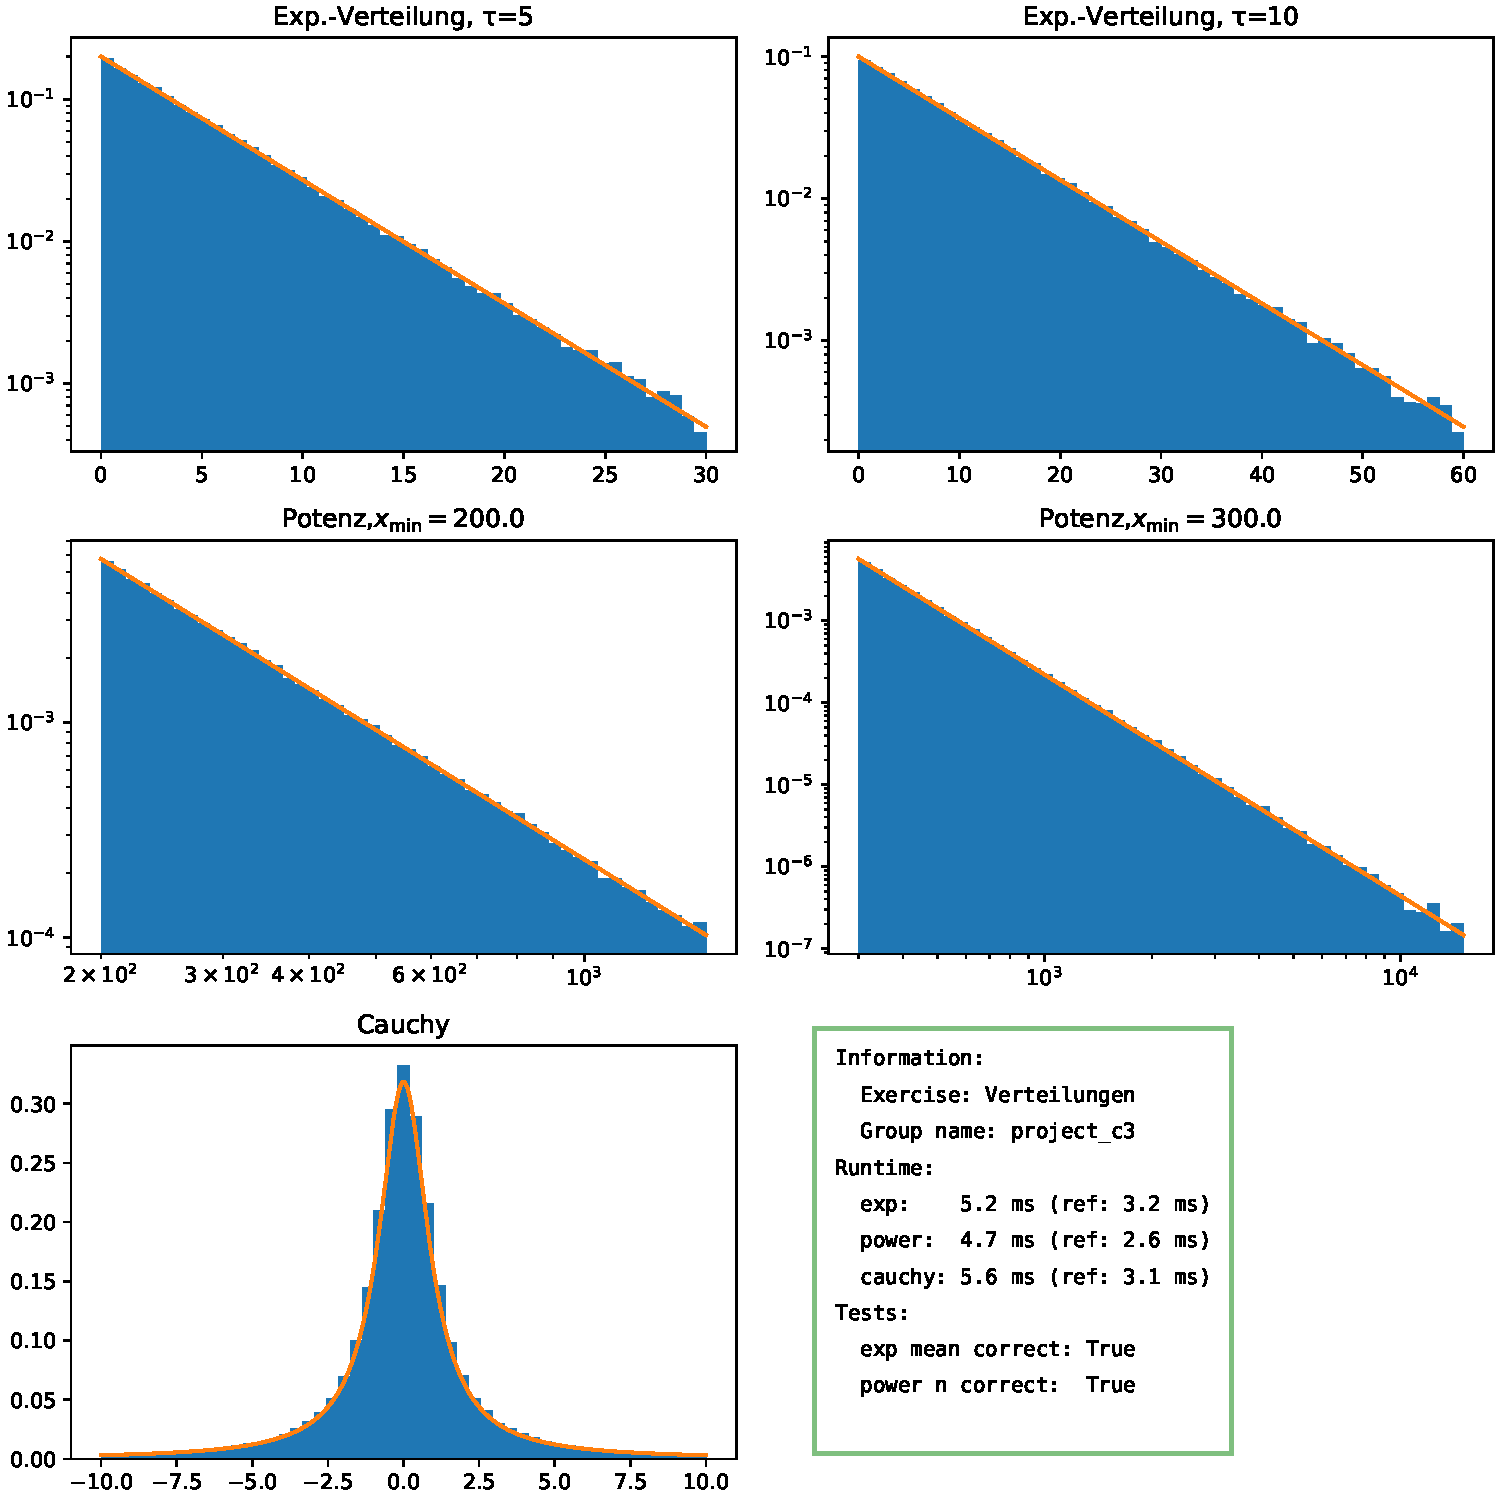
\includegraphics[width=\textwidth]{distributions.pdf}
		\caption{Ergebnis der Testdatei.}
	\end{figure}

\end{document}
